\documentclass[english, letterpaper, 10 pt]{report}

\usepackage{color}
\usepackage[T1]{fontenc}
\usepackage{multirow}
\usepackage{caption}
\usepackage{float}
\usepackage{hyperref}
\usepackage{cleveref}
\usepackage{listings}
\usepackage{graphicx}
\usepackage[export]{adjustbox}
\graphicspath{ {pictures/user-documentation} }
\hypersetup{
    colorlinks,
    linktoc=all,
    citecolor=black,
    filecolor=black,
    linkcolor=black,
    urlcolor=black
}

% -------------------------------------------------------------------------------------
% BEGIN DOCUMENT
% -------------------------------------------------------------------------------------
\begin{document}
\title{User Documentation}
\author{Philip Rebbe \\
Sarah Julia Kriesch}
\maketitle
\pagestyle{empty}


\newpage
% -------------------------------------------------------------------------------------
% Getting started
% ------------------------------------------
% -------------------------------------------
\section*{Getting started}

Clone the current version of the repository or download the executable version of the latest \href{https://github.com/amosproj/amos2022ss08-openid-connect-doctor/releases}{release} from GitHub. If you clone the repository, make sure, that you have installed a sufficient Node.js-version.


% -------------------------------------------------------------------------------------
% Examining an identity-provider
% -------------------------------------------------------------------------------------
\section*{Examining an identity-provider}

\subsection* {Starting an application}

There are two ways to start the application:

\begin{enumerate}
\item If you cloned the repository, you can run one of the build-scripts located in the root directory of the repository to start the application. They will install all necessary dependencies for the project and start the application with \textit{npm start}. 
\item If you downloaded the latest release, you just have to start the downloaded executable. This will open a terminal window displaying the internal logs of the application. \\ \textbf{Hint:} There is a need to download or clone the views, schema, public and log files directories from the project. The binary has to be placed on top of all these directories.
\end{enumerate}    

\noindent When the application is started, it will automatically open a new browser tab, and will redirect you to the start page of the application.
\\

\noindent \textbf{Important:} If no browser tab is opened, open a new browser window and enter \url{http://localhost:8081/} to navigate to the main page.
\\
\begin{figure}[H]
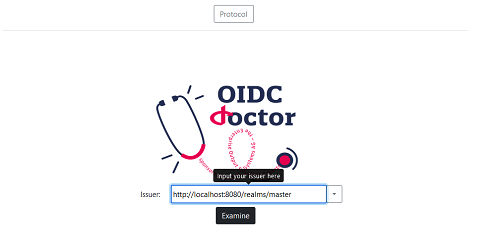
\includegraphics[scale=0.9,frame]{StartPageScreenshot.png}
\caption{Start Page Example}
\end{figure}
\newpage
\subsection*{Checking the discovery-endpoint}

\noindent To start the examination of the discovery-endpoint, enter the URL of the identity-provider you want to examine and hit the \textit{Examine}-Button (Make sure that you input the correct base-URL if the identity-provider is deployed in sub-directory for example).

\noindent If you provided a valid endpoint the application will then direct you to a result-page displaying the contents of the providers discovery-endpoint. This page contains some options to filter and validate the displayed informations and export the result as a text-file:
\begin{itemize}
\item To filter the output, open the advanced settings and click on the \textit{filter}-button. This will open a dialog, that lets you select the values, that should be displayed.
\item To validate the displayed information, open the advanced settings and choose one of the provided JSON-schemas:
\begin{itemize}
\item If the endpoint contains the required information, the result of the endpoint are displayed and the found values are highlighted.
\item If the endpoint does not contain all required information, the validation fails and the missing values are displayed in the output of the result page.
\end{itemize}
\item To copy or export the result of the discovery-endpoint, simply click on the corresponding buttons.
\end{itemize}
\newpage
\textbf{Hints:}
\begin{itemize}
\item In case you don't have a specific identity-provider, that you want to test, you can also select one of the default options provided in the dropdown menu next to the input field. Simply choose one of the provided options and the input-field will be set to the select provider.
\item If you already have a token and want to skip the rest of the examination, simply click on the button at the bottom of the site to skip to the \textit{ \nameref{Decode-Token}} step.
\end{itemize}

\begin{figure}[H]
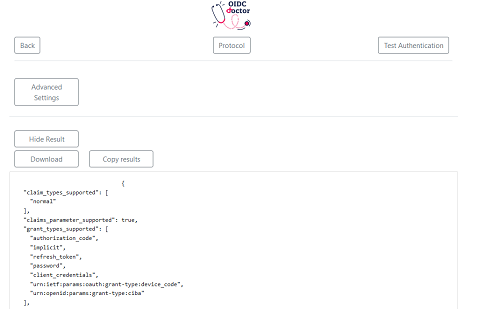
\includegraphics[scale=0.8,frame]{DiscoveryResultScreenshot.png}
\caption{Discovery Result}
\end{figure}

\subsection*{Testing the authentication-flows}

\noindent The next step after testing the contents of the discovery-endpoint is to check the authentication-flows that are provided by the identity-provider.
\\

\noindent \textbf{Important:} Most of these flows have the requirement, that the openid-connect-doctor is registered at the identity-provider as client-application! Please follow the official documentation of the identity-provider if you need more information on how to register a client-application.
\\

\noindent To see, which flows are available for the identity-provider, click on the \textit{Test Authentication}-button in the top right corner of the application. This will redirect you to an overview-page that shows all flows that can currently be tested with the openid-doctor. The following options are currently available:
\begin{itemize}
\item Client-Credential-Flow
\item Password-Grant-Flow
\item Authorization-Code-Flow
\end{itemize}

\noindent All options provide a short description of the flow and are enabled/disabled based on the previously requested discovery-information, to make sure these options only show the currently available flows. The available options are highlighted with a green border and the unavailable flows are hightlighted with a red border.
\\
\begin{figure}[H]
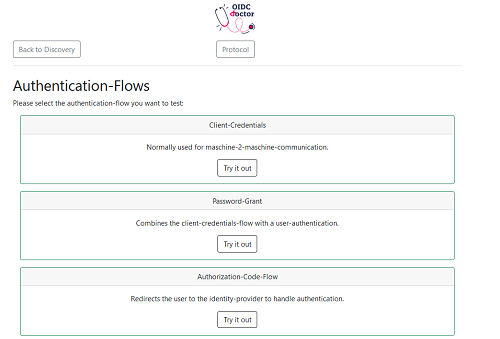
\includegraphics[scale=0.8,frame]{AuthenticationFlowsOverviewScreenshot.png}
\caption{Overview about Authentication Flows}
\end{figure}


\noindent If you want to test one of these flows, click on the \textit{Try it out}-button below the description. This will redirect you to an input-mask, that asks you for the information that are required to request an access-token via this flow. In case of the client-credentials-flow for example, this includes the URL of the identity-provider (prefilled), the client-id and -secret of the openid-connect-doctor that were set, when registering the app as a client-application and the optional audience parameter (see the image below).
\newpage

\noindent After you have entered the necessary information, you can click on the \textit{Submit}-button to send the request to the identity-provider. The application will then request an access token and redirect you to the token-decode-page, where you can analyze the token.
\\
\begin{figure}[H]
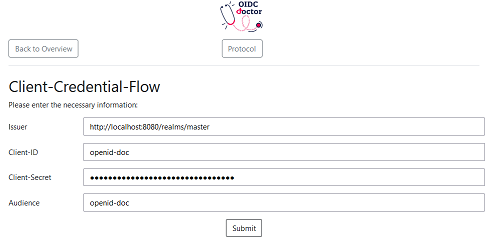
\includegraphics[scale=0.8,frame]{ClientCredentialsFlowInputScreenshot.png}
\caption{Client Credential Flow Input}
\end{figure}

\subsection*{Decoding an access-token} \label{Decode-Token}

\noindent At last you want to decode the returned access-token and check if all the relevant headers and claims are available. For this you can navigate to \url{http://localhost:8081/api/token/decode}. This will display a input-mask, where you can enter the url of the identity-provider that issued the token and the access-token (if you used one of the authenication-flows from the previous section, the issuer and access-token are already set). Below the two text-fields are some additional settings, that can be used to filter and validate the information from the access-token:
\begin{itemize}
\item To validate the header or the payload of the token, open the advanced settings, select the header- or token-settings and choose one of the provided schemas from the dropdown menu. If a schema is chosen, the content of the access-token is automatically validated against the schema, when the input is submitted. If all the values are available in the section, the validation succeeds and the values are highlighted. If some values are missing, the validation fails and the missing values are displayed instead of the output.
\item Per default the signature of the access-token is validate against the key-material of the issuer. If you want to use a local key-file to validate the signature, open the signature-section of the advanced settings and untick the option to use the key-material of the jwks-endpoint. After that enter the filepath to the keyfile and the hash-algorithm to calculate the signature into the two text-fields below. The validation will then try to access the keyfile to validate the signature.
\end{itemize}


\noindent If you have entered all the necessary information, click on the \textit{Submit}-Button to start the decoding and validation of the access-token. The result is then displayed below the input fields, along with a short message describing the result of the validation. The results can then be downloaded or copied via the corresponding buttons.
\\
\begin{figure}[H]
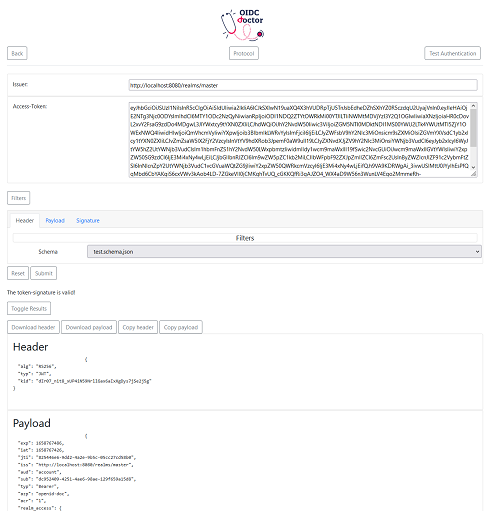
\includegraphics[scale=0.8,frame]{TokenDecodeScreenshot.png}
\caption{Decode a Token}
\end{figure}
\newpage

\subsection*{Configuring the application}

\noindent If you are using the source-code-version of the application, you can use the json-file located at \texttt{./settings/default.json} to enable/disable some functions of the application. This may come in handy if your identity-provider is configured to restrict the result of the discovery-endpoint or if you only are interested in some of the values shown on the discovery-page. The following settings are available:

\begin{table}[h!]
  \begin{center}
  \captionof{table}{Application Configuration Settings}
    \begin{tabular}{|c|c|c|p{6cm}|} % <-- Alignments: 1st column left, 2nd middle and 3rd right, with vertical lines in between
    \hline
      \textbf{section} & \textbf{Parameter} & \textbf{Data Type} & \textbf{Description}\\
      \hline
      Discovery & Parameter & String-Array & Controls the values that are shown when the discovery-endpoint is triggered for the first time.\\ \hline
      Discovery & \verb|validation_schema| & String & Sets the default-schema for the validation of the discovery-result.\\ \hline
      Token & \verb|validation_schema| & String & Sets the default-schema for the validation of the token-header and payload.\\ \hline
      Token & \verb|key_algorithm| & String & Sets the default-key-algorithm for the validaiton of the token-signature.\\ \hline
      Flows & \verb|always_on| & String-Array & Specifies the authentication-flows, that are always enabled, even if they are not specified as supported by the discovery-endpoint\\ \hline
      Flows & \verb|always_off| & String-Array & Specifies the authentication-flows, that are always disabled, even if they are specified as supported by the discovery-endpoint\\ \hline
    \end{tabular}
  \end{center}
\end{table}


\subsection*{Accessing the protocol}

\noindent If the information display during one of the steps are not detailed enough, you can access the more detailed protocol information via the \textit{Protocol}-button that is displayed in the header of the application. This will redirect you to a separate page that contains detailed information about the last 50 requests including timestamps, status-codes and server-side-error-messages.
\\

\noindent \textbf{Disclaimer:} All screenshots were created via Greenshot\footnote{https://github.com/greenshot/greenshot} and while testing a local docker-container running keycloak\footnote{https://www.keycloak.org}.

% -------------------------------------------------------------------------------------
% REFERENCES
% -------------------------------------------------------------------------------------
%\bibliography{}

% -------------------------------------------------------------------------------------
% END DOCUMENT
% -------------------------------------------------------------------------------------
\end{document}
